\documentclass[11pt,a4paper]{article}

\usepackage[a4paper,margin=25mm]{geometry}
\usepackage[T1]{fontenc}
\usepackage[utf8]{inputenc}
\usepackage{lmodern}
\usepackage{microtype}
\usepackage{graphicx}
\usepackage{booktabs}
\usepackage{array}
\usepackage{longtable}
\usepackage{tabularx}
\usepackage{multirow}
\usepackage{float}
\usepackage{caption}
\usepackage{subcaption}
\usepackage{amsmath,amssymb}
\usepackage{siunitx}
\usepackage{enumitem}
\usepackage{fancyhdr}
\usepackage{titlesec}
\usepackage{xcolor}
\usepackage{tikz}
\usepackage{hyperref}
\usepackage{url}
\usepackage{setspace}
\usepackage{lastpage}
\usepackage{etoolbox}

\graphicspath{{assets/}}
\hypersetup{colorlinks=true,linkcolor=black,citecolor=black,urlcolor=blue,pdftitle={Finite Element Stress Analysis of a Mechanical Plate}}
\captionsetup{font=small,labelfont=bf}
\setstretch{1.12}
\setlength{\parskip}{0.4em}
\setlength{\parindent}{0pt}
\setlist[itemize]{topsep=2pt,itemsep=2pt,leftmargin=6mm}
\setlist[enumerate]{topsep=2pt,itemsep=2pt,leftmargin=7mm}
\sisetup{group-separator={,},group-minimum-digits=4}
\setlength{\headheight}{14pt}

\definecolor{ujorange}{HTML}{F36F21}
\definecolor{ujdark}{HTML}{1F2937}
\definecolor{ujgray}{HTML}{6B7280}

\titleformat{\section}{\Large\bfseries\color{ujdark}}{\thesection}{0.6em}{}
\titleformat{\subsection}{\large\bfseries\color{ujdark}}{\thesubsection}{0.6em}{}

\pagestyle{fancy}
\fancyhf{}
\lhead{Finite Element Stress Analysis of a Mechanical Plate}
\rhead{Strength of Materials 4A}
\cfoot{Page \thepage\ of \pageref{LastPage}}
\renewcommand{\headrulewidth}{0.4pt}
\renewcommand{\footrulewidth}{0pt}

\newcommand{\reporttitle}{Finite Element Stress Analysis of a Mechanical Plate}
\newcommand{\studentname}{Sithabiso Msane}
\newcommand{\studentnumber}{223180282}
\newcommand{\modulecode}{Strength of Materials 4A - Assessment 3}
\newcommand{\department}{Department of Mechanical Engineering Science}
\newcommand{\faculty}{Faculty of Engineering and the Built Environment}
\newcommand{\software}{SOLIDWORKS Simulation}

\begin{document}

\begin{titlepage}
\begin{tikzpicture}[remember picture,overlay]
  \fill[ujorange] (current page.north west) rectangle ([yshift=-42mm]current page.north east);
  \fill[ujorange!12] ([xshift=0mm,yshift=-42mm]current page.north west) rectangle ([xshift=18mm]current page.south west);
  \draw[ujorange,line width=1.1pt] ([xshift=18mm,yshift=-58mm]current page.north west) -- ([xshift=-18mm,yshift=-58mm]current page.north east);
  \draw[ujorange,line width=1.1pt] ([xshift=18mm,yshift=35mm]current page.south west) -- ([xshift=-18mm,yshift=35mm]current page.south east);
\end{tikzpicture}

\vspace*{12mm}
{\color{white}\bfseries\fontsize{20}{22}\selectfont UNIVERSITY OF JOHANNESBURG\par}
\vspace{2mm}
{\color{white}\large \faculty\par}
\vspace{16mm}

{\Huge\bfseries\color{ujdark}\reporttitle\par}
\vspace{4mm}
{\Large\color{ujgray}\modulecode\par}
\vspace{8mm}

{\large This report presents the finite element modelling, mesh convergence study, and final static stress results for the mechanical plate specified in the assignment brief. The selected solution was obtained using a converged mesh with local refinement at the stress concentration zones.\par}

\vfill

\begin{tabular}{>{\bfseries}p{45mm}p{95mm}}
Student Name: & \studentname \\
Student Number: & \studentnumber \\
Software: & \software \\
Module: & \modulecode \\
Department: & \department \\
Date: & \today \\
\end{tabular}

\vfill

{\small\color{ujgray}Prepared in \LaTeX\ with figures extracted from the supplied \software\ result reports and plots generated from the uploaded mesh refinement study.\par}
\end{titlepage}

\tableofcontents
\clearpage

\section{Introduction}

\subsection{Background}
The finite element method (FEM) is a standard engineering tool for estimating stresses, strains, and deformations in components with irregular geometry and complex load paths. Instead of relying only on closed-form formulae, the continuum is discretized into a set of elements connected at nodes, and the governing equilibrium problem is solved numerically in the form
\begin{equation}
    [K]\{u\}=\{F\},
\end{equation}
where $[K]$ is the global stiffness matrix, $\{u\}$ is the nodal displacement vector, and $\{F\}$ is the applied load vector \cite{logan2016,cook2001,zienkiewicz2013}.

For plate-like parts containing holes, relief cut-outs, and abrupt changes in section, the local stress field is not uniform. Instead, stress concentrations develop near the geometric discontinuities, and these peaks must be captured with sufficient mesh density to avoid misleading numerical results \cite{pilkey2008,khechai2014}. A mesh convergence study is therefore essential: the mesh is progressively refined until the key response quantities become essentially unchanged. This is the point at which the numerical model is considered stable and reliable \cite{barnkopf2023}.

In the present assignment, the part is a \SI{12}{mm}-thick plate with one large circular opening and two semicircular relief features. The left face is fixed and a \SI{3000}{N} normal load is applied to the right-hand face. The objective is to determine the mass of the part, the maximum von Mises stress, the largest expected compressive stress, the maximum horizontal displacement, and the numerical size of the finite element model.

\subsection{Aim}
The aim of this report is to perform a static linear-elastic finite element stress analysis of the mechanical plate and to select a numerically efficient mesh that produces converged results for the required output quantities.

\subsection{Objectives}
The specific objectives were to:
\begin{enumerate}
    \item model the supplied plate geometry in \software;
    \item assign the material properties specified in the assignment;
    \item apply the prescribed fixed support and distributed load;
    \item perform a static finite element analysis for a sequence of progressively refined meshes;
    \item compute the degrees of freedom (DOF) for each model;
    \item compare stress and displacement convergence trends; and
    \item select and justify the final mesh used for reporting the assignment results.
\end{enumerate}

\subsection{Report Overview}
Section 2 defines the finite element model, including the geometry, boundary conditions, loading, material data, acceptance criteria, and discretization strategy. Section 3 presents the finite element results, convergence plots, contour plots, and the final summary table. The report concludes with the main findings, followed by the references and appendices.

\section{Finite Element Model}

\subsection{Geometry}
The final CAD model used for the analysis is shown in Fig.~\ref{fig:geometry}. The plate thickness is \SI{12}{mm}, and the model image indicates that the student-number-based circular feature diameter used in the final part is \SI{82}{mm}. The geometry also contains an upper semicircular cut-out and a lower semicircular relief, which are expected to act as local stress raisers.

\begin{figure}[H]
    \centering
    \begin{subfigure}[t]{0.48\textwidth}
        \centering
        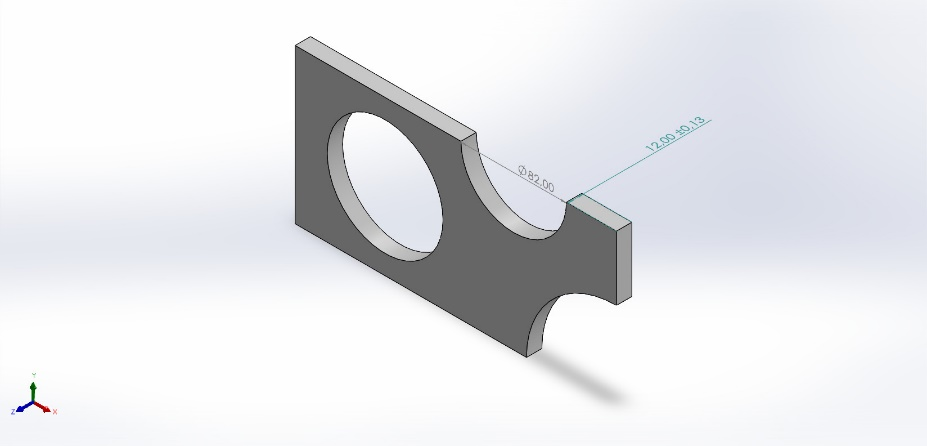
\includegraphics[width=\linewidth]{model_geometry.jpeg}
        \caption{Final geometric model used in the analysis.}
    \end{subfigure}
    \hfill
    \begin{subfigure}[t]{0.48\textwidth}
        \centering
        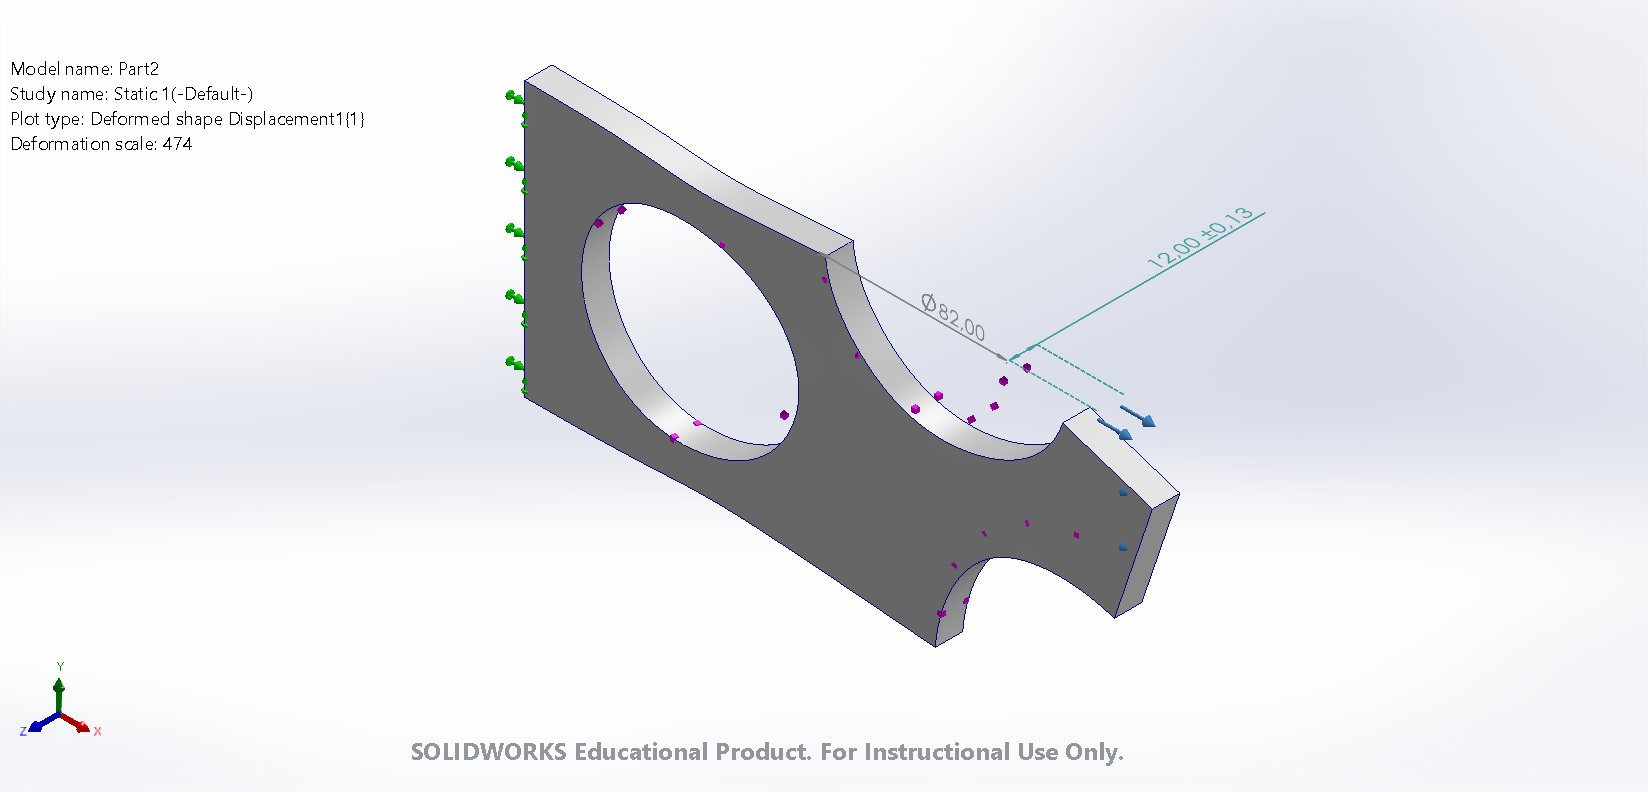
\includegraphics[width=\linewidth]{bc_loads.jpg}
        \caption{Model with fixed support and applied face load.}
    \end{subfigure}
    \caption{Geometric representation of the analysed plate.}
    \label{fig:geometry}
\end{figure}

\subsection{Boundary conditions}
The left-hand face of the plate was fully constrained using a fixed geometry support. This suppresses translation in all three global directions on that face and creates a cantilever-type response. The support representation is visible in Fig.~\ref{fig:geometry}(b).

\subsection{Loads}
A normal force of \SI{3000}{N} was applied to the loaded face on the right-hand side of the part. The load was distributed over the face rather than applied at a point, which is consistent with the assignment brief and avoids an artificial point-load singularity.

\subsection{Analysis}
A static linear-elastic analysis was performed using 3D solid elements in \software. Small-displacement behaviour was assumed, and the response was taken as purely mechanical. The required output quantities were extracted directly from the solution reports:
\begin{itemize}
    \item maximum von Mises stress;
    \item largest expected compressive stress, taken as the magnitude of the minimum third principal stress;
    \item maximum horizontal displacement, taken from the maximum positive $U_X$ value; and
    \item resultant displacement, used only as a secondary convergence check.
\end{itemize}

\subsection{Material properties}
The assignment specified a linear elastic isotropic material with modulus of elasticity $E=\SI{190}{GPa}$, Poisson's ratio $\nu=0.29$, and density $\rho=\SI{7800}{kg.m^{-3}}$. These properties were used to evaluate stiffness and mass. The SolidWorks material card used in the final report also contained a yield strength of \SI{250}{MPa}, which was used only as a practical acceptance check for the final von Mises stress result.

\begin{table}[H]
    \centering
    \caption{Material properties used in the finite element model.}
    \begin{tabular}{ll}
        \toprule
        Property & Value \\
        \midrule
        Elastic modulus, $E$ & \SI{190}{GPa} \\
        Poisson's ratio, $\nu$ & 0.29 \\
        Density, $\rho$ & \SI{7800}{kg.m^{-3}} \\
        Yield strength, $\sigma_y$ (material card) & \SI{250}{MPa} \\
        \bottomrule
    \end{tabular}
    \label{tab:material}
\end{table}

\subsection{Acceptance criteria}
The final model was accepted only if it satisfied the following engineering checks:
\begin{enumerate}
    \item \textbf{Force equilibrium:} the resultant reaction force should closely match the applied load of \SI{3000}{N}.
    \item \textbf{Mesh convergence:} the key outputs should show negligible change relative to the finest uniform mesh. In this report, a change below \SI{1}{\percent} in both maximum von Mises stress and maximum horizontal displacement was used as the practical threshold.
    \item \textbf{Elastic stress limit:} the final maximum von Mises stress should remain below the assigned yield strength of \SI{250}{MPa}.
\end{enumerate}

The factor of safety against first yield for the final selected mesh is estimated by
\begin{equation}
    n_y = \frac{\sigma_y}{\sigma_{\mathrm{vm,max}}} = \frac{250}{49.06} \approx 5.10.
\end{equation}

\subsection{Discretization}
A blended curvature-based solid mesh was used. Uniform global mesh sizes of \SIlist{14;10;8;5;3;2;1}{mm} were tested first. After the convergence trends were established, a final mesh was created using a global size of \SI{8}{mm} together with a local mesh control of \SI{2}{mm} on three faces around the stress concentration regions. This strategy was adopted to keep the model computationally efficient while preserving solution accuracy in the critical areas.

For a 3D solid model with translational degrees of freedom only, the total number of degrees of freedom is approximated by
\begin{equation}
    \mathrm{DOF} = 3\,N_{\mathrm{nodes}}.
\end{equation}

The final selected mesh is shown in Fig.~\ref{fig:mesh}.

\begin{figure}[H]
    \centering
    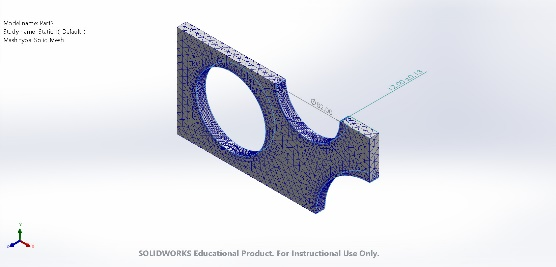
\includegraphics[width=0.60\textwidth]{final_mesh.jpeg}
    \caption{Final converged mesh used for reporting, with global element size of \SI{8}{mm} and local mesh control of \SI{2}{mm}.}
    \label{fig:mesh}
\end{figure}

\section{Results}

\subsection{Finite element results}
The mesh refinement study showed clear convergence of the key response quantities. As the uniform mesh was refined from \SI{14}{mm} to \SI{1}{mm}, the maximum von Mises stress increased from \SI{47.40}{MPa} to \SI{49.05}{MPa}, while the maximum horizontal displacement changed only from \SI{0.05189}{mm} to \SI{0.05217}{mm}. The response therefore stabilised strongly once the mesh size reached about \SI{3}{mm}.

The final controlled mesh produced a maximum von Mises stress of \SI{49.06}{MPa}, a largest compressive stress of \SI{31.63}{MPa}, and a maximum horizontal displacement of \SI{0.05216}{mm}. These values are effectively identical to the \SI{1}{mm} uniform-mesh solution, while the final selected model required only \num{43116} nodes and \num{129348} DOF instead of \num{1947481} nodes and \num{5842443} DOF. This is a major reduction in computational cost with negligible loss of accuracy.

The final model also satisfied the equilibrium check: the reaction force reported by the solver was \SI{2999.94}{N}, which differs from the applied load by only about \SI{0.002}{\percent}. The selected model is therefore both converged and mechanically consistent.

\begin{figure}[H]
    \centering
    \begin{subfigure}[t]{0.48\textwidth}
        \centering
        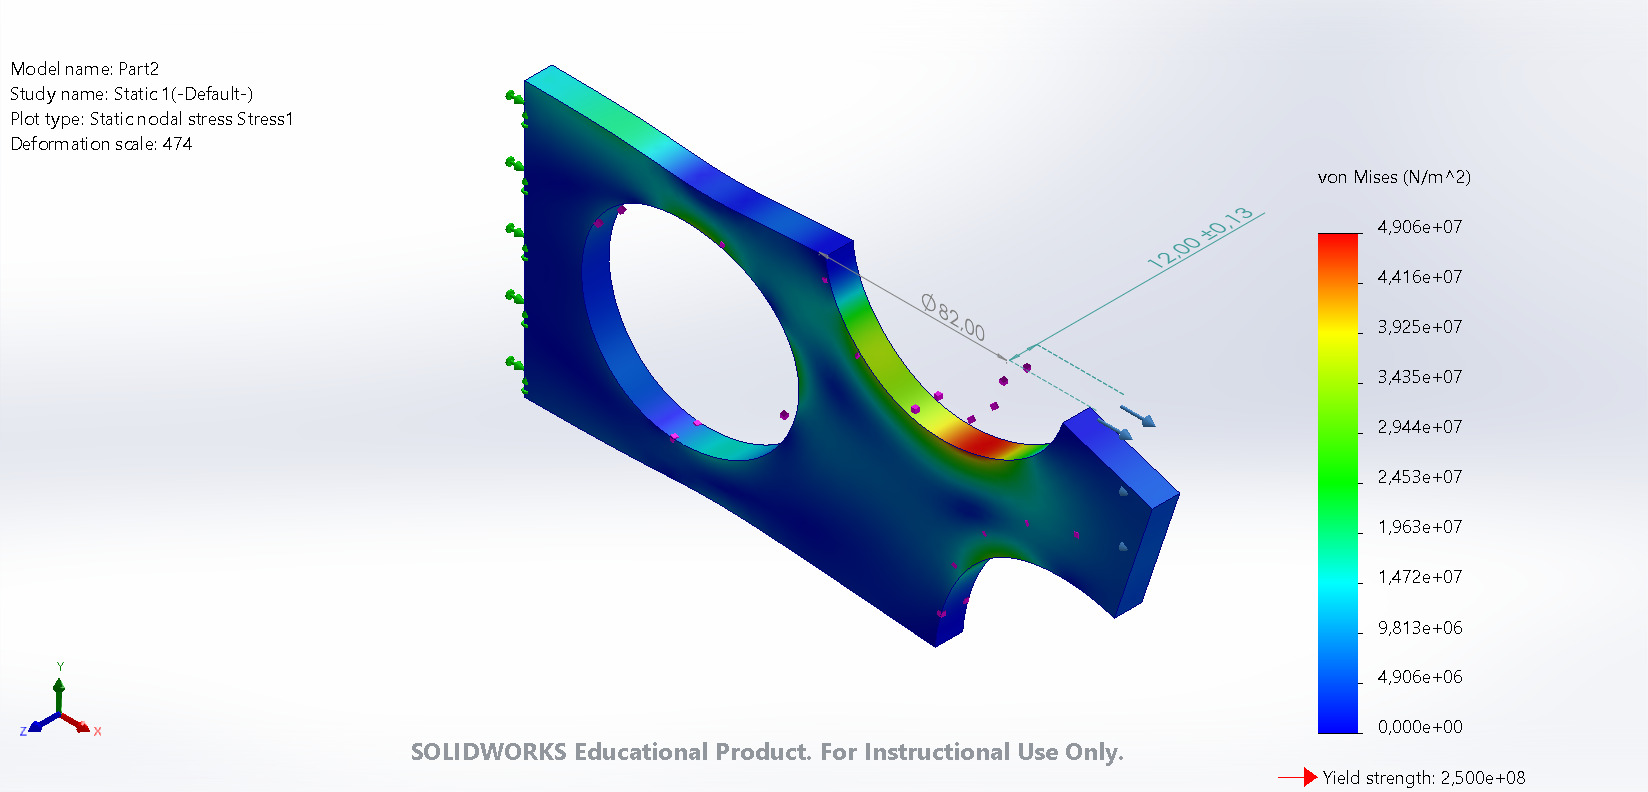
\includegraphics[width=\linewidth]{von_mises_contour.jpg}
        \caption{von Mises stress contour.}
    \end{subfigure}
    \hfill
    \begin{subfigure}[t]{0.48\textwidth}
        \centering
        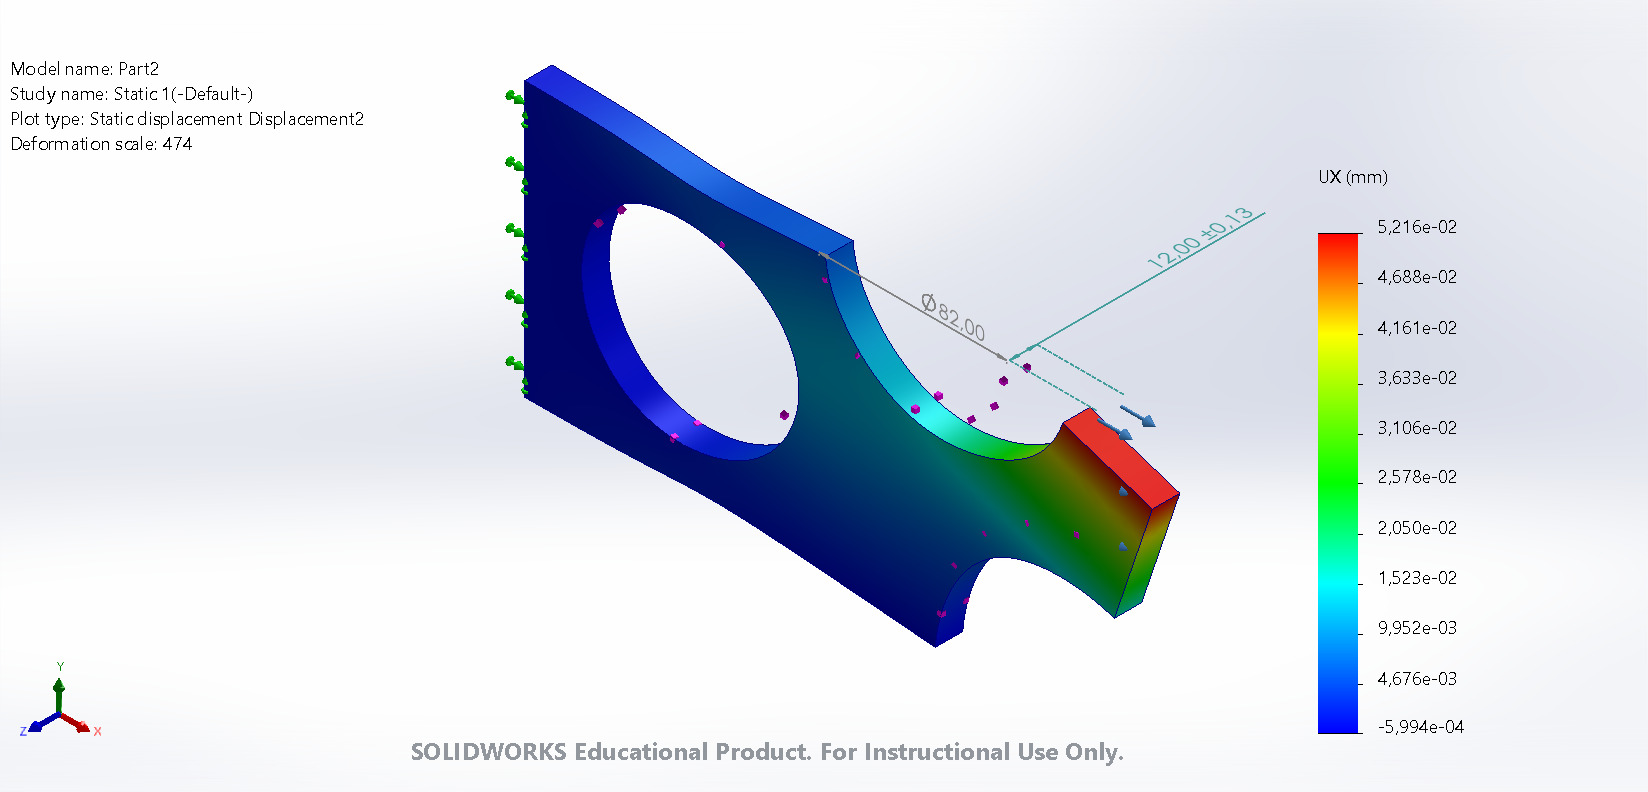
\includegraphics[width=\linewidth]{ux_contour.jpg}
        \caption{Horizontal displacement ($U_X$) contour.}
    \end{subfigure}
    \caption{Primary results from the final converged model. The peak von Mises stress occurs at the upper relief transition, while maximum horizontal displacement occurs at the loaded end.}
    \label{fig:primaryresults}
\end{figure}

\begin{figure}[H]
    \centering
    \begin{subfigure}[t]{0.48\textwidth}
        \centering
        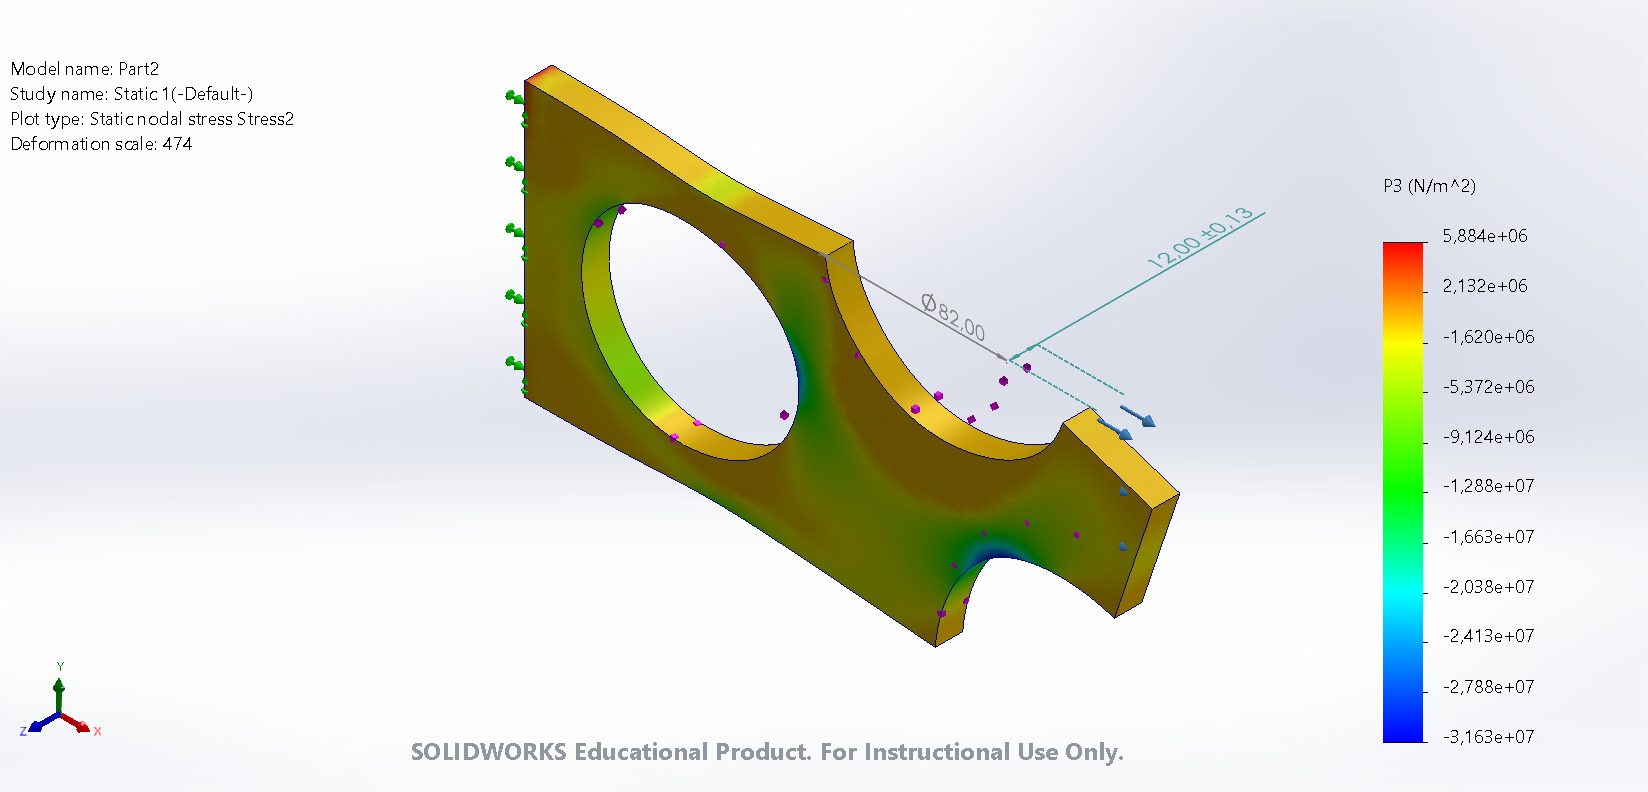
\includegraphics[width=\linewidth]{p3_contour.jpg}
        \caption{Third principal stress ($P_3$) contour.}
    \end{subfigure}
    \hfill
    \begin{subfigure}[t]{0.48\textwidth}
        \centering
        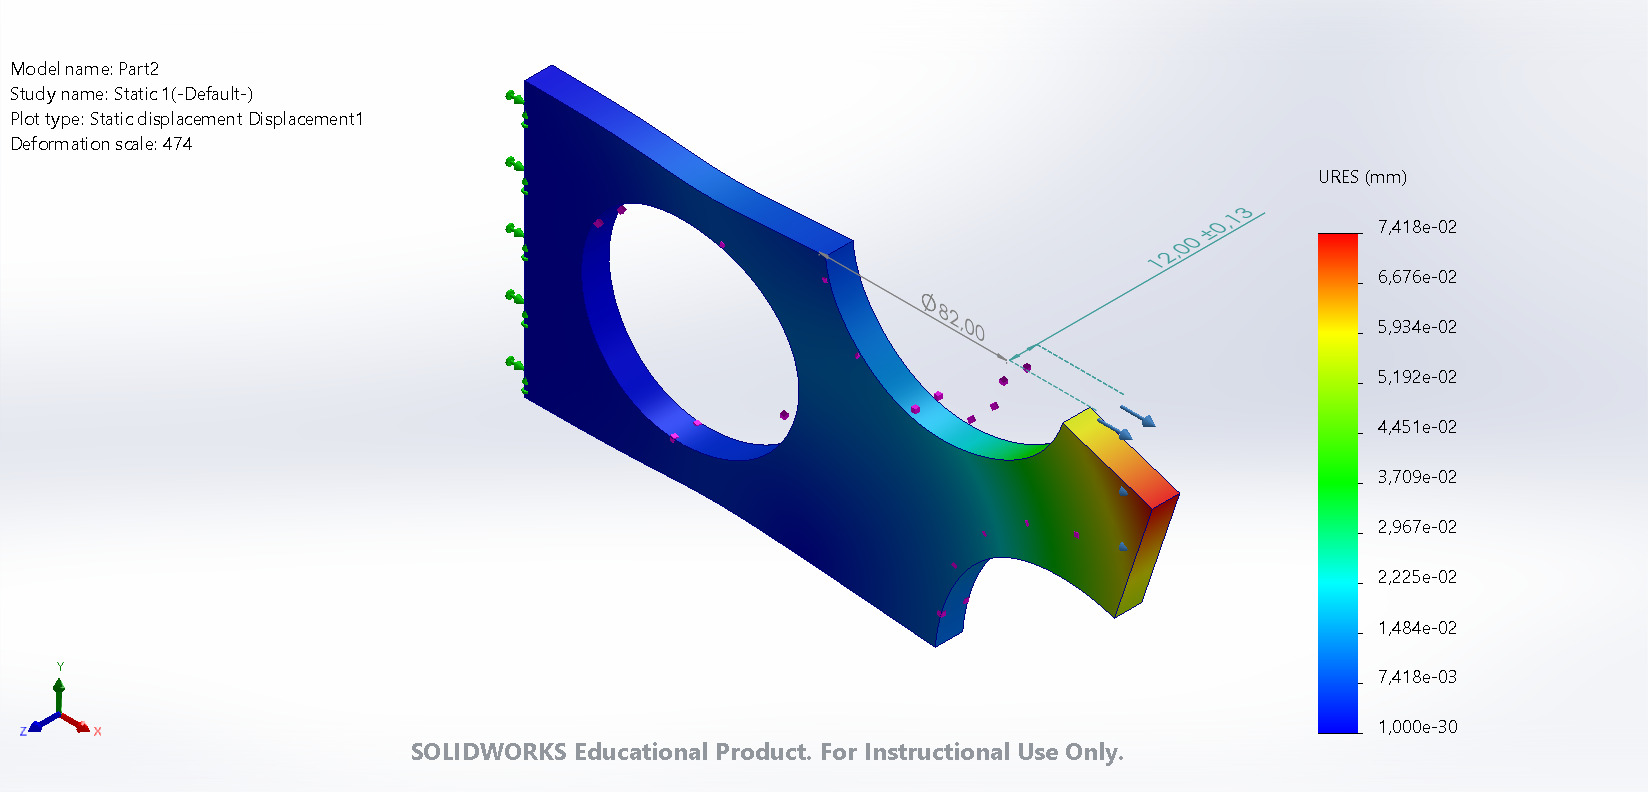
\includegraphics[width=\linewidth]{resultant_displacement_contour.jpg}
        \caption{Resultant displacement contour.}
    \end{subfigure}
    \caption{Additional result fields from the final selected mesh. The most severe compressive stress is associated with the minimum $P_3$ region near the lower relief feature.}
    \label{fig:secondaryresults}
\end{figure}

\begin{figure}[H]
    \centering
    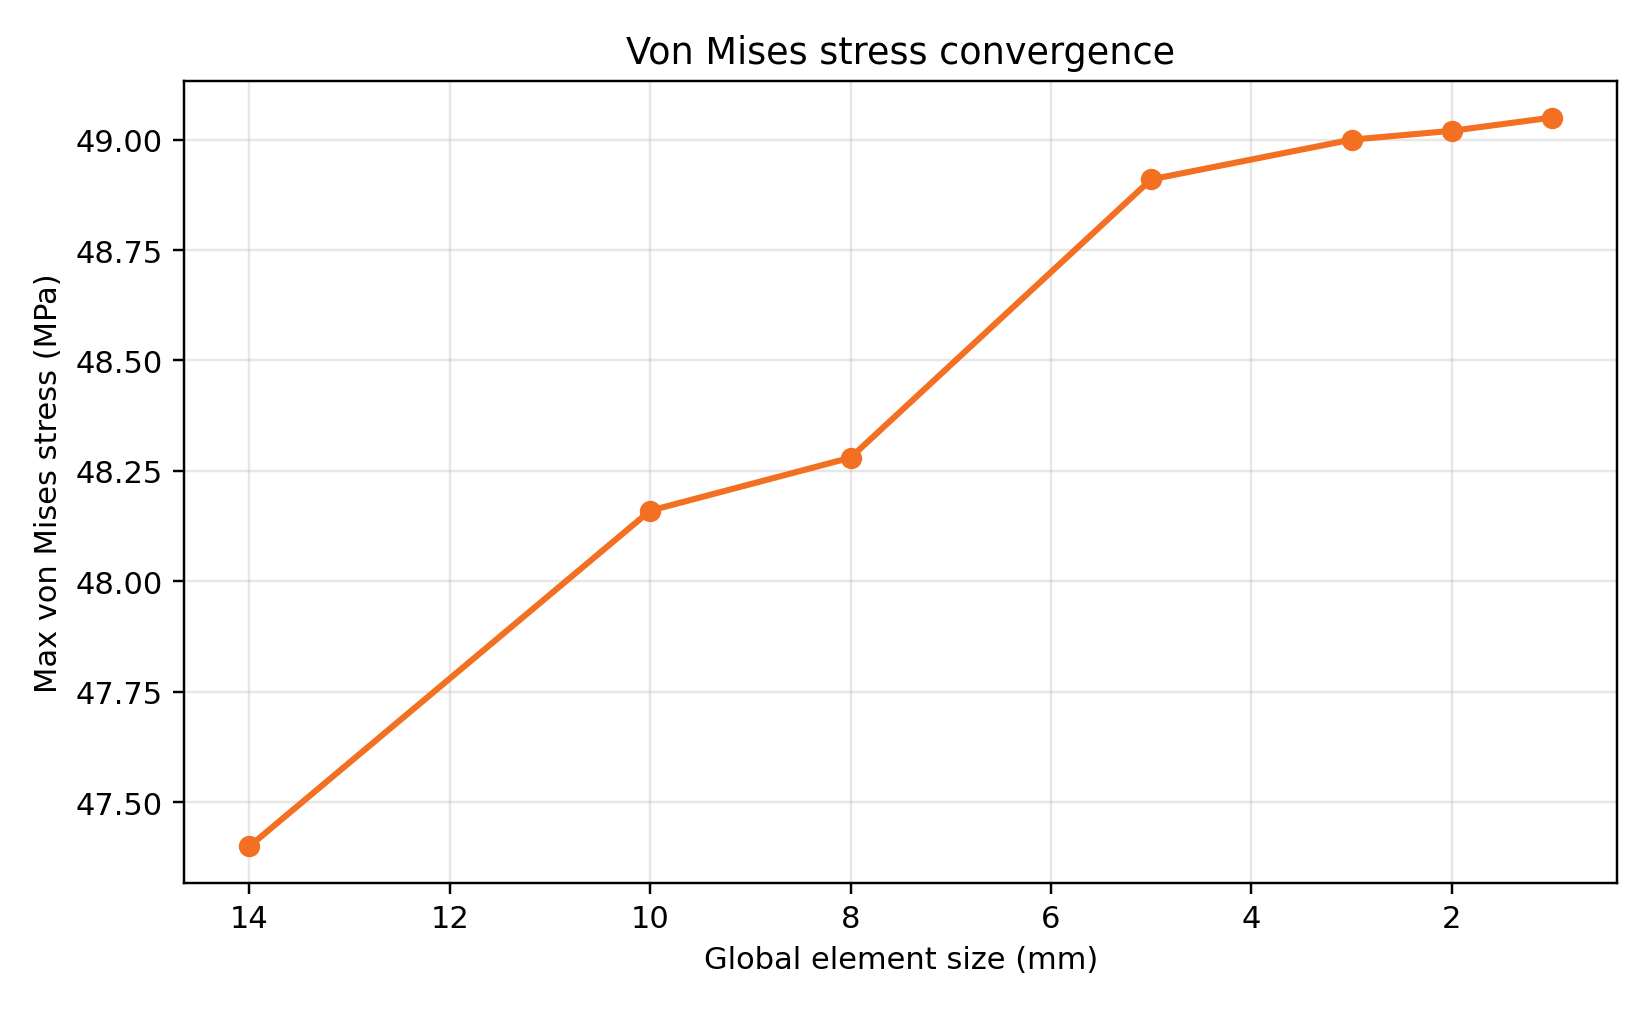
\includegraphics[width=0.83\textwidth]{plot_vm_convergence.png}
    \caption{Convergence of maximum von Mises stress with progressive mesh refinement.}
    \label{fig:vmplot}
\end{figure}

\begin{figure}[H]
    \centering
    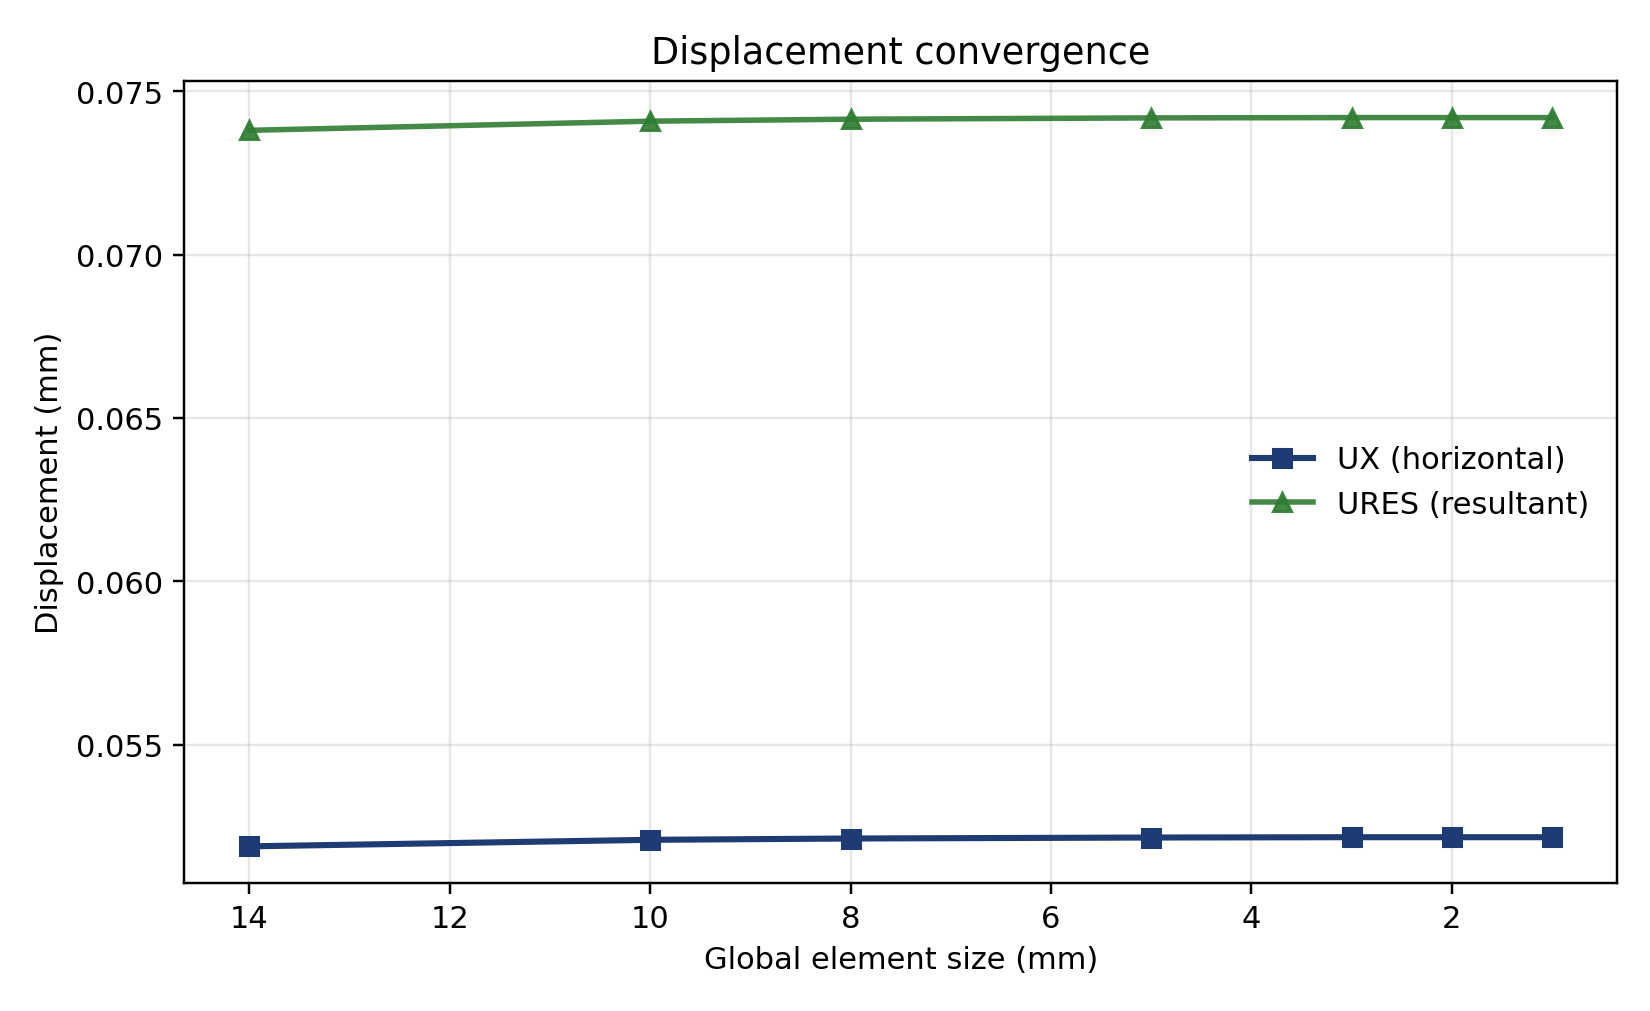
\includegraphics[width=0.83\textwidth]{plot_displacement_convergence.png}
    \caption{Convergence of maximum horizontal and resultant displacement. The assignment quantity of interest is the horizontal displacement $U_X$.}
    \label{fig:uxplot}
\end{figure}

\begin{figure}[H]
    \centering
    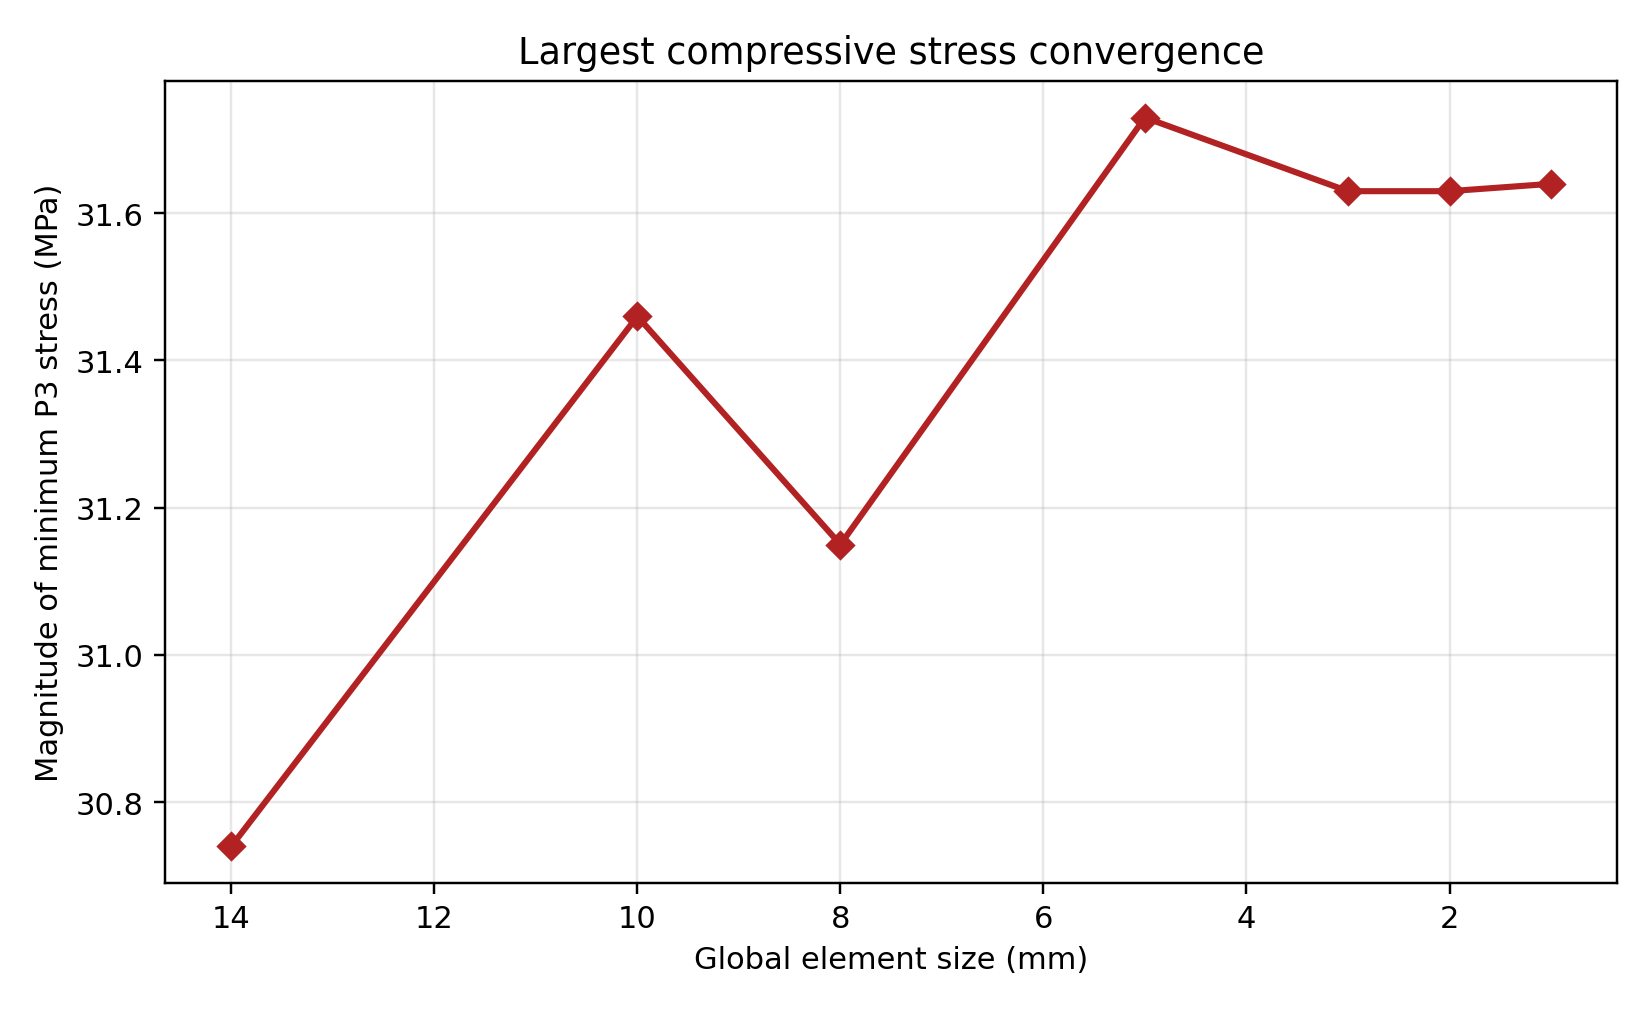
\includegraphics[width=0.83\textwidth]{plot_p3_convergence.png}
    \caption{Convergence of the magnitude of the minimum third principal stress, interpreted here as the largest expected compressive stress.}
    \label{fig:p3plot}
\end{figure}

\begin{figure}[H]
    \centering
    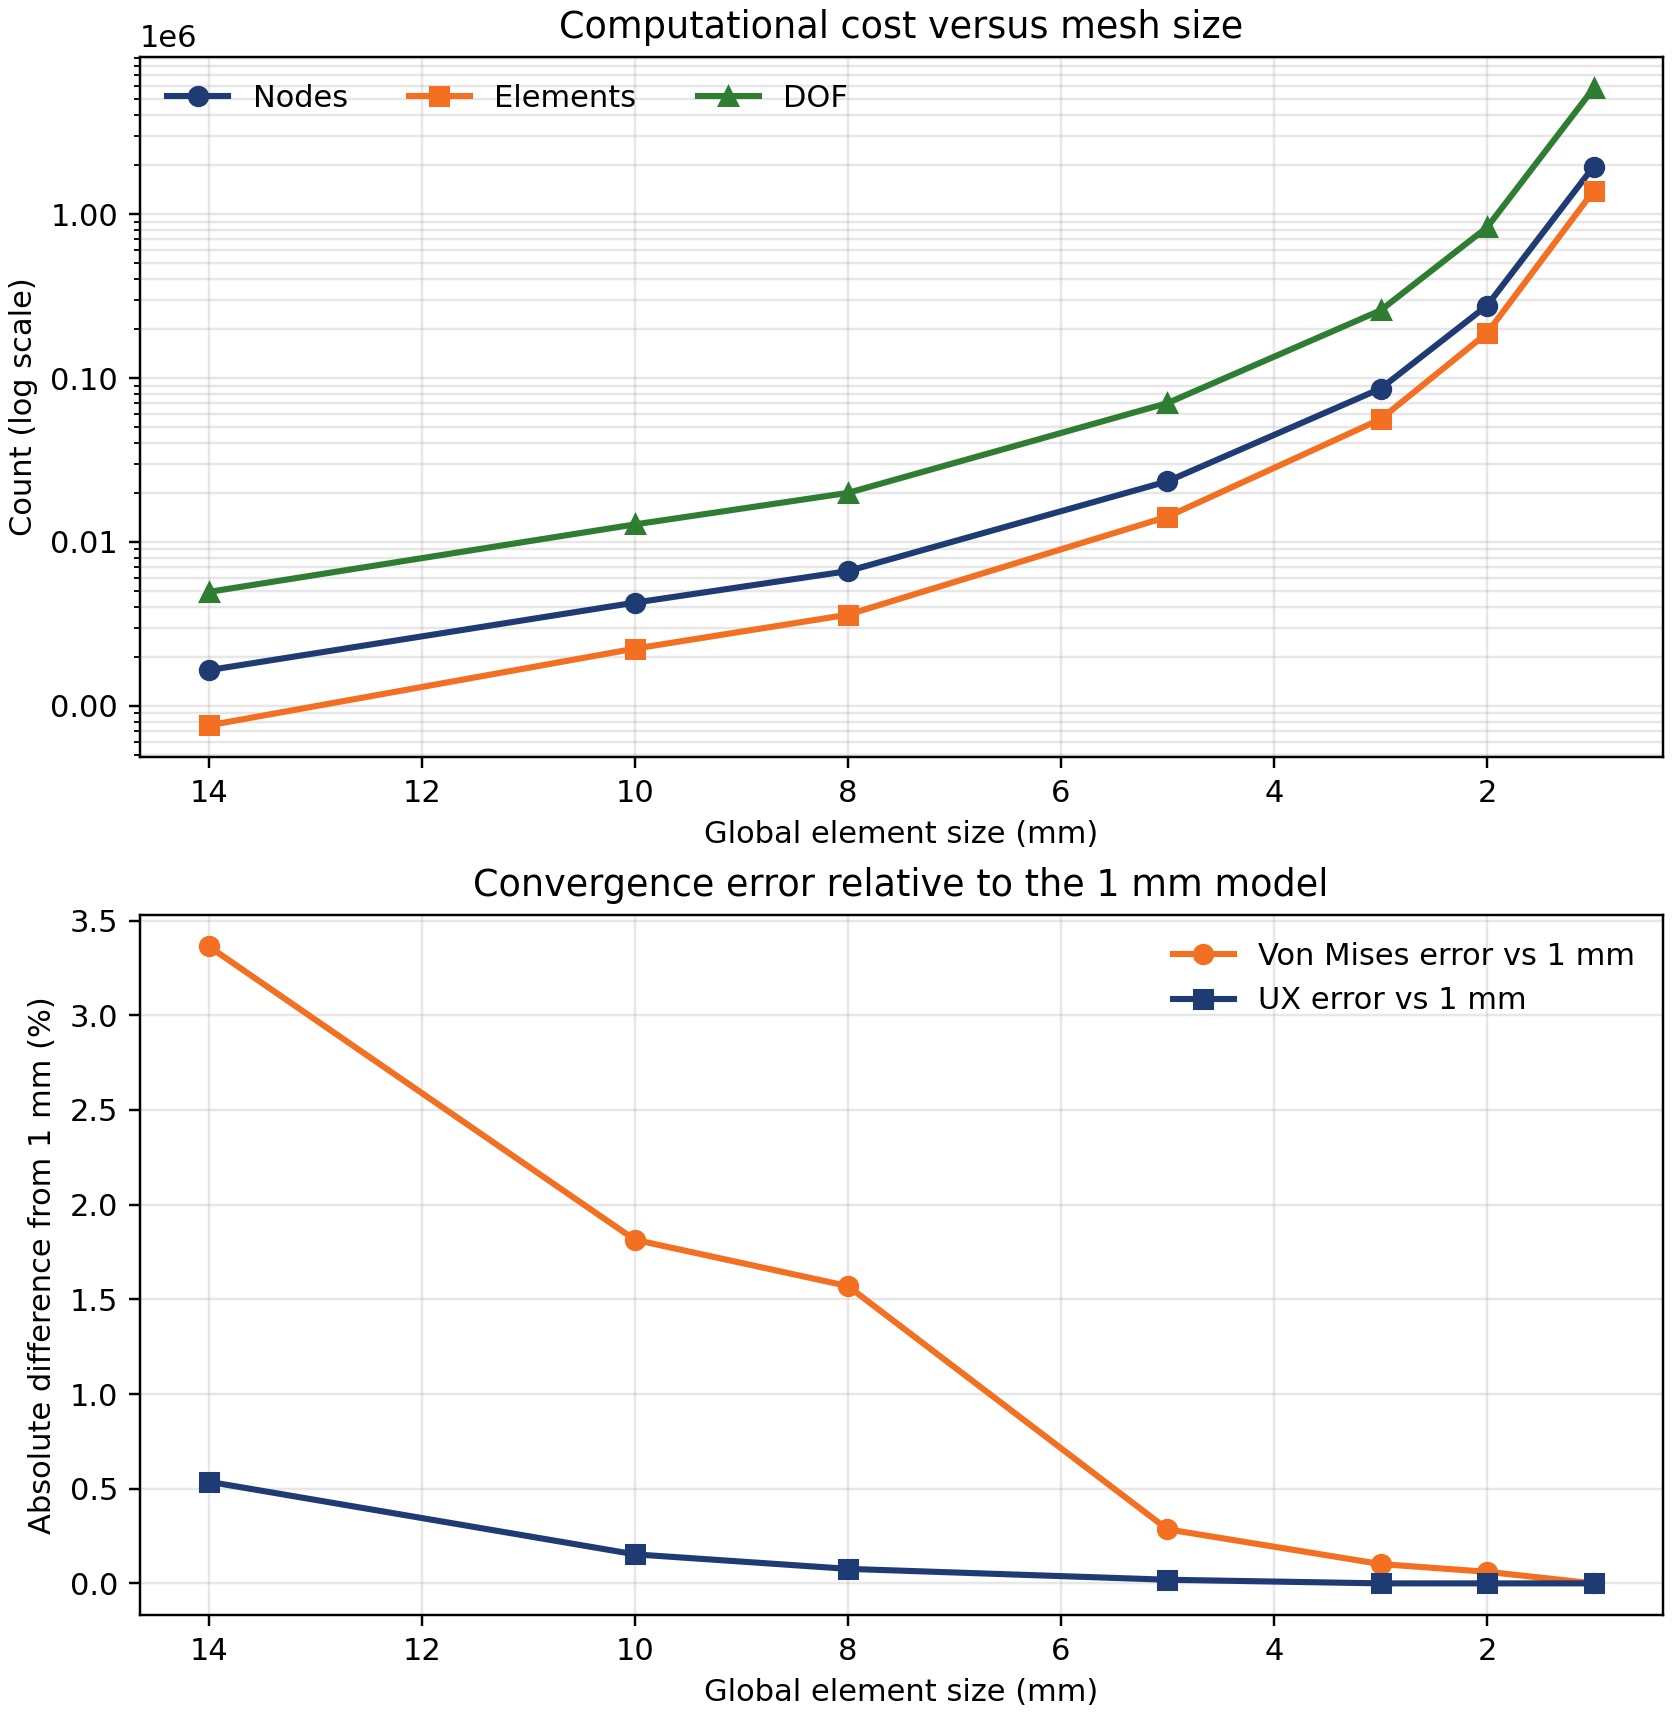
\includegraphics[width=0.86\textwidth]{plot_mesh_cost_error.png}
    \caption{Computational cost and convergence error trends for the uniform mesh study. The final selected controlled mesh achieved near-fine-mesh accuracy without the full cost penalty of the \SI{1}{mm} model.}
    \label{fig:costplot}
\end{figure}

\subsection{Summary / table of results}
Table~\ref{tab:summary} gives the final reported values for the selected converged mesh. These are the values recommended for direct inclusion in the assignment table.

\begin{table}[H]
    \centering
    \caption{Final reported values for the selected mesh (\SI{8}{mm} global + \SI{2}{mm} local control).}
    \begin{tabular}{>{\raggedright\arraybackslash}p{85mm}r}
        \toprule
        Quantity & Value \\
        \midrule
        Student number & \studentnumber \\
        Mass of part & \SI{1.605}{kg} \\
        Maximum stress (von Mises) & \SI{49.06}{MPa} \\
        Largest expected compressive stress & \SI{31.63}{MPa} \\
        Maximum horizontal displacement ($U_X$) & \SI{0.05216}{mm} \\
        Number of nodes & \num{43116} \\
        Number of elements & \num{21530} \\
        Degrees of freedom & \num{129348} \\
        \bottomrule
    \end{tabular}
    \label{tab:summary}
\end{table}

For completeness, Table~\ref{tab:convergence} summarizes the entire convergence study. The mass remained constant because the geometry and material density were unchanged, while the stress and displacement outputs approached asymptotic values as the mesh became finer.

\begin{table}[H]
    \centering
    \caption{Mesh refinement results and calculated degrees of freedom.}
    \label{tab:convergence}
    {\small
    \setlength{\tabcolsep}{4pt}%
    \resizebox{\textwidth}{!}{%
    \begin{tabular}{lrrrrrrr}
        \toprule
        Mesh case & Nodes & Elements & DOF & $\sigma_{\mathrm{vm,max}}$ (MPa) & $|P_{3,\min}|$ (MPa) & $U_X$ (mm) & $U_{\mathrm{res}}$ (mm)\\
        \midrule
        14 mm uniform & 1653 & 761 & 4959 & 47.40 & 30.74 & 0.05189 & 0.07380 \\
        10 mm uniform & 4265 & 2236 & 12795 & 48.16 & 31.46 & 0.05209 & 0.07408 \\
        8 mm uniform & 6640 & 3602 & 19920 & 48.28 & 31.15 & 0.05213 & 0.07414 \\
        5 mm uniform & 23443 & 14260 & 70329 & 48.91 & 31.73 & 0.05216 & 0.07418 \\
        3 mm uniform & 86136 & 56077 & 258408 & 49.00 & 31.63 & 0.05217 & 0.07419 \\
        2 mm uniform & 276481 & 187931 & 829443 & 49.02 & 31.63 & 0.05217 & 0.07419 \\
        1 mm uniform & 1947481 & 1384266 & 5842443 & 49.05 & 31.64 & 0.05217 & 0.07419 \\
        8 mm global + 2 mm control & 43116 & 21530 & 129348 & 49.06 & 31.63 & 0.05216 & 0.07418 \\
        \bottomrule
    \end{tabular}}}
\end{table}

\section{Conclusion}
A static finite element stress analysis was completed for the mechanical plate using \software. The mesh refinement study showed clear convergence of the main output quantities. The maximum von Mises stress converged to approximately \SI{49}{MPa}, the largest compressive stress converged to approximately \SI{31.6}{MPa}, and the maximum horizontal displacement converged to approximately \SI{0.0522}{mm}.

The final selected mesh --- a global element size of \SI{8}{mm} with a local \SI{2}{mm} mesh control in the stress concentration regions --- is the best engineering choice for this assignment. It reproduces the fine-mesh results almost exactly, while using only a small fraction of the nodes, elements, and degrees of freedom required by the \SI{1}{mm} uniform mesh. The final reported results are therefore numerically justified, mechanically consistent, and computationally efficient.

\bibliographystyle{ieeetr}
\bibliography{references}

\appendix
\clearpage
\section{Additional notes on reported quantities}
\begin{itemize}
    \item The \textbf{largest expected compressive stress} was taken as the magnitude of the minimum third principal stress, because compression appears as a negative principal stress in the SolidWorks reports.
    \item The \textbf{maximum horizontal displacement} required by the assignment was taken from the maximum positive $U_X$ value, not from the resultant displacement magnitude.
    \item The \textbf{degrees of freedom} were calculated as three translational DOF per node for the 3D solid model.
\end{itemize}

\section{Why the final mesh was selected}
The final controlled mesh was selected because it provides essentially the same response as the finest uniform mesh but at much lower computational cost. Relative to the \SI{1}{mm} uniform mesh, the selected model differs by only about \SI{0.02}{\percent} in maximum von Mises stress and about \SI{0.02}{\percent} in maximum horizontal displacement, yet it reduces the DOF from \num{5842443} to \num{129348}. That trade-off is highly favorable for engineering report work, where accuracy and efficiency both matter.

\end{document}
